\documentclass[aspectratio=43,11pt]{beamer}
\usetheme{default}
\usecolortheme{default}
\setbeamertemplate{navigation symbols}{}
\setbeamertemplate{footline}[frame number]
%\setbeamercolor{structure}{fg=black}
\setbeamercolor{structure}{fg=aggiemaroon}
%\setbeamercolor{frametitle}{fg=black,bg=black!6}
\setbeamercolor{frametitle}{fg=aggiemaroon} %,bg=aggiemaroon!0
\setbeamerfont{frametitle}{series=\bfseries}
\usepackage{booktabs}
\usepackage{amsmath}
\usepackage{listings}
\usepackage{xcolor}
\usepackage{pgfplots}
\pgfplotsset{compat=1.18}
\definecolor{priorblue}{RGB}{49,95,160}
\definecolor{datagreen}{RGB}{36,130,90}
\definecolor{postred}{RGB}{180,65,55}
\definecolor{aggiemaroon}{RGB}{80,0,0}

%\documentclass[aspectratio=43,11pt]{beamer}

% ============================================================
% Packages
% ============================================================
\usepackage{amsmath}
\usepackage{booktabs}
\usepackage{tikz}

\usetikzlibrary{
  arrows.meta,
  positioning,
  shapes.geometric
}

% ============================================================
% Beamer appearance
% ============================================================
%\usetheme{Madrid}
\usecolortheme{default}

\definecolor{dagblue}{RGB}{38,91,150}
\definecolor{daggreen}{RGB}{55,130,95}
\definecolor{dagorange}{RGB}{210,120,35}
\definecolor{dagred}{RGB}{175,55,55}
\definecolor{daggray}{RGB}{90,95,105}

%\setbeamercolor{structure}{fg=dagblue}
%\setbeamercolor{alerted text}{fg=dagred}
\setbeamertemplate{navigation symbols}{}

% ============================================================
% TikZ styles
%
% The "dag" prefixes prevent conflicts with predefined TikZ keys.
% ============================================================
\tikzset{
  dagNode/.style={
    circle,
    draw=dagblue,
    fill=dagblue!10,
    thick,
    minimum size=1.15cm,
    align=center
  },
  dagObserved/.style={
    circle,
    draw=daggreen,
    fill=daggreen!18,
    thick,
    minimum size=1.15cm,
    align=center
  },
  dagDecision/.style={
    rectangle,
    rounded corners=1pt,
    draw=dagorange,
    fill=dagorange!15,
    thick,
    minimum width=1.45cm,
    minimum height=0.9cm,
    align=center
  },
  dagUtility/.style={
    diamond,
    draw=dagred,
    fill=dagred!12,
    thick,
    aspect=1.5,
    minimum width=1.6cm,
    align=center
  },
  dagArrow/.style={
    -{Latex[length=2.5mm]},
    thick,
    draw=daggray
  }
}

% ============================================================
% Title information
% ============================================================
%\title{Directed Acyclic Graphs}
%\subtitle{A Friendly Introduction to DAGs, Bayesian Networks, and Decisions}
%\author{Alexander}
%\institute{Texas A\&M University}
%\date{}

\title{Decision and Risk Analysis}
\subtitle{Lecture 4 p1: \textbf{Directed Acyclic Graphs, Bayesian Balance and Sequential Learning}}
\author{\emph{}}
\date{\color{aggiemaroon}{
DAEN 427 / ISEN 427 / ISEN 627\\
\textbf{Alexander Abuabara}\\
Fall 2026
}}
\titlegraphic{\vfill 
\includegraphics[height=1.2cm]{TAMU_logo.png}}

% ============================================================
\begin{document}
% ============================================================

% ------------------------------------------------------------
\begin{frame}
  \titlepage
\end{frame}

% ------------------------------------------------------------
\begin{frame}{The basic idea}

A \alert{directed acyclic graph}, usually called a \textbf{DAG},
contains:

\begin{itemize}
  \item \textbf{Nodes}: things we care about;
  \item \textbf{Arrows}: directed relationships;
  \item \textbf{No directed cycles}: we cannot follow arrows and return
        to where we started.
\end{itemize}

\medskip

\begin{center}
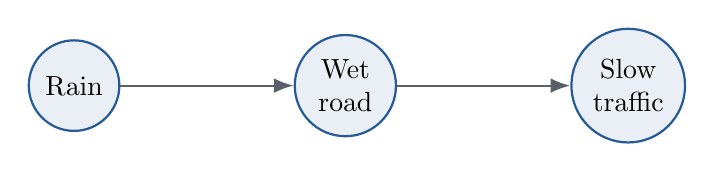
\begin{tikzpicture}[node distance=2.2cm]
  \node[dagNode] (rain) {Rain};

  \node[dagNode, right=of rain]
    (road) {Wet\\road};

  \node[dagNode, right=of road]
    (traffic) {Slow\\traffic};

  \draw[dagArrow] (rain) -- (road);
  \draw[dagArrow] (road) -- (traffic);
\end{tikzpicture}
\end{center}

\medskip

Informally, we read this as

\[
\text{Rain}
\longrightarrow
\text{Wet road}
\longrightarrow
\text{Slow traffic}.
\]

\end{frame}

% ------------------------------------------------------------
\begin{frame}{Why ``acyclic''?}

This is a DAG:

\begin{center}
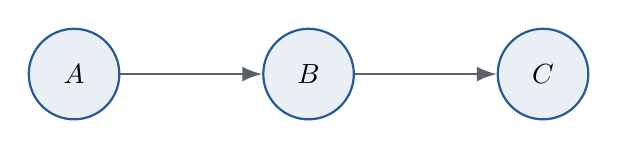
\begin{tikzpicture}[node distance=1.8cm]
  \node[dagNode] (a1) {$A$};
  \node[dagNode, right=of a1] (b1) {$B$};
  \node[dagNode, right=of b1] (c1) {$C$};

  \draw[dagArrow] (a1) -- (b1);
  \draw[dagArrow] (b1) -- (c1);
\end{tikzpicture}
\end{center}

But this is \alert{not} a DAG:

\begin{center}
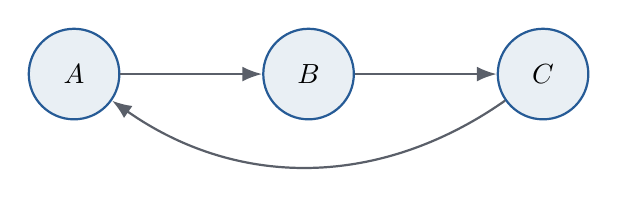
\begin{tikzpicture}[node distance=1.8cm]
  \node[dagNode] (a2) {$A$};
  \node[dagNode, right=of a2] (b2) {$B$};
  \node[dagNode, right=of b2] (c2) {$C$};

  \draw[dagArrow] (a2) -- (b2);
  \draw[dagArrow] (b2) -- (c2);
  \draw[dagArrow, bend left=35] (c2) to (a2);
\end{tikzpicture}
\end{center}

Following the arrows produces the directed cycle

\[
A \longrightarrow B \longrightarrow C \longrightarrow A.
\]

\end{frame}

% ------------------------------------------------------------
\begin{frame}{Some family vocabulary}

\begin{center}
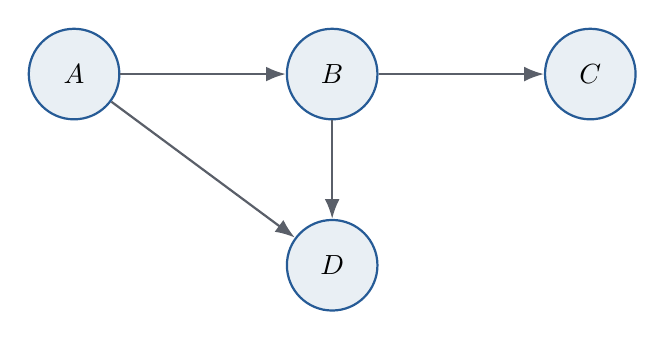
\begin{tikzpicture}[node distance=2.1cm]
  \node[dagNode] (a) {$A$};
  \node[dagNode, right=of a] (b) {$B$};
  \node[dagNode, right=of b] (c) {$C$};
  \node[dagNode, below=1.25cm of b] (d) {$D$};

  \draw[dagArrow] (a) -- (b);
  \draw[dagArrow] (b) -- (c);
  \draw[dagArrow] (a) -- (d);
  \draw[dagArrow] (b) -- (d);
\end{tikzpicture}
\end{center}

Relative to \(B\):

\begin{itemize}
  \item \(A\) is a \textbf{parent} of \(B\);
  \item \(C\) and \(D\) are \textbf{children} of \(B\);
  \item \(A\) is an \textbf{ancestor} of \(C\) and \(D\);
  \item \(C\) and \(D\) are \textbf{descendants} of \(A\).
\end{itemize}

A valid \textbf{topological ordering} is \(A,B,C,D\).

\end{frame}

% ------------------------------------------------------------
\begin{frame}{What does an arrow mean?}

An arrow \(X\rightarrow Y\) does not have one universal meaning.

\begin{block}{Depending on the application, it may represent}
\begin{itemize}
  \item a computational dependency;
  \item a prerequisite;
  \item a temporal relationship;
  \item direct probabilistic dependence;
  \item or a causal effect.
\end{itemize}
\end{block}

\pause

\begin{alertblock}{Important warning}
A DAG is causal only when the arrows are assigned a causal
interpretation and the required assumptions are defensible.
\end{alertblock}

\medskip

Correlation alone does not tell us which way an arrow should point.

\end{frame}

% ------------------------------------------------------------
\begin{frame}{Three patterns worth remembering}

\begin{columns}[T]

\column{0.32\textwidth}
\centering

\textbf{Chain}

\medskip

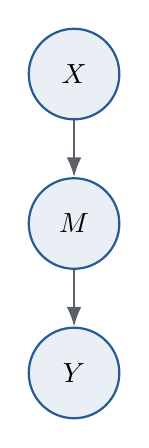
\begin{tikzpicture}[node distance=0.72cm]
  \node[dagNode] (x1) {$X$};
  \node[dagNode, below=of x1] (m1) {$M$};
  \node[dagNode, below=of m1] (y1) {$Y$};

  \draw[dagArrow] (x1) -- (m1);
  \draw[dagArrow] (m1) -- (y1);
\end{tikzpicture}

\[
X\rightarrow M\rightarrow Y
\]

\column{0.32\textwidth}
\centering

\textbf{Fork}

\medskip

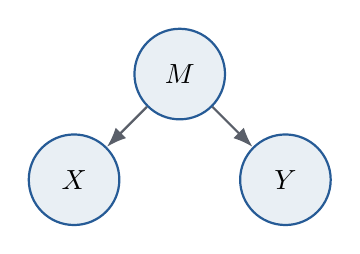
\begin{tikzpicture}[node distance=0.72cm]
  \node[dagNode] (m2) {$M$};
  \node[dagNode, below left=of m2] (x2) {$X$};
  \node[dagNode, below right=of m2] (y2) {$Y$};

  \draw[dagArrow] (m2) -- (x2);
  \draw[dagArrow] (m2) -- (y2);
\end{tikzpicture}

\[
X\leftarrow M\rightarrow Y
\]

\column{0.32\textwidth}
\centering

\textbf{Collider}

\medskip

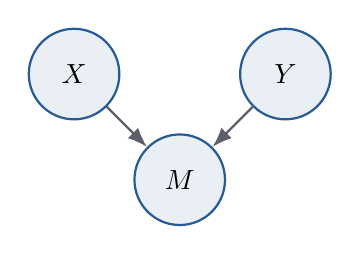
\begin{tikzpicture}[node distance=0.72cm]
  \node[dagNode] (m3) {$M$};
  \node[dagNode, above left=of m3] (x3) {$X$};
  \node[dagNode, above right=of m3] (y3) {$Y$};

  \draw[dagArrow] (x3) -- (m3);
  \draw[dagArrow] (y3) -- (m3);
\end{tikzpicture}

\[
X\rightarrow M\leftarrow Y
\]

\end{columns}

\medskip

These patterns behave differently when we condition on \(M\).

\end{frame}

% ------------------------------------------------------------
\begin{frame}{Conditioning can block or open a path}

\begin{table}
\centering
\begin{tabular}{lll}
\toprule
\textbf{Pattern} & \textbf{Normally} & \textbf{Given \(M\)} \\
\midrule
\(X\rightarrow M\rightarrow Y\)
  & Path open & Path blocked \\[2mm]

\(X\leftarrow M\rightarrow Y\)
  & Path open & Path blocked \\[2mm]

\(X\rightarrow M\leftarrow Y\)
  & Path blocked & Path opened \\
\bottomrule
\end{tabular}
\end{table}

\medskip

The collider is the surprising case.

\begin{exampleblock}{Informal example}
Ability and family connections may both affect admission:

\[
\text{Ability}
\longrightarrow
\text{Admission}
\longleftarrow
\text{Connections}.
\]

Among admitted students, ability and connections may appear related even
if they are unrelated in the general population.
\end{exampleblock}

\end{frame}

% ------------------------------------------------------------
\begin{frame}{D-separation, informally}

\textbf{D-separation} is a graphical test for deciding whether two sets
of variables are conditionally independent.

\medskip

A path is blocked when:

\begin{enumerate}
  \item it contains a chain or fork whose middle node is conditioned on; or
  \item it contains a collider, unless the collider or one of its
        descendants is conditioned on.
\end{enumerate}

\medskip

If every path between \(X\) and \(Y\) is blocked by \(Z\), then the DAG
implies

\[
X \perp\!\!\!\perp Y \mid Z.
\]

\begin{block}{Plain-language interpretation}
After we know \(Z\), learning \(X\) gives us no additional information
about \(Y\).
\end{block}

\end{frame}

% ------------------------------------------------------------
\begin{frame}{From a DAG to a Bayesian network}

A \textbf{Bayesian network} combines:

\begin{enumerate}
  \item a DAG describing local dependencies; and
  \item a probability distribution for each node given its parents.
\end{enumerate}

\begin{center}
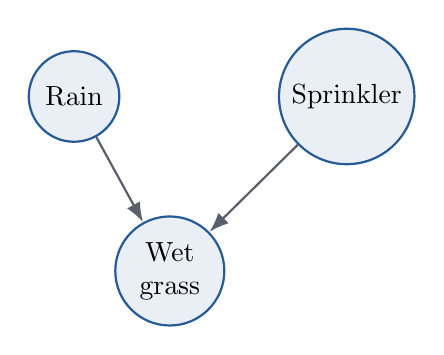
\begin{tikzpicture}[node distance=2cm]
  \node[dagNode] (rain2) {Rain};

  \node[dagNode, right=of rain2]
    (sprinkler) {Sprinkler};

  \node[dagNode, below right=1.3cm and 0.3cm of rain2]
    (grass) {Wet\\grass};

  \draw[dagArrow] (rain2) -- (grass);
  \draw[dagArrow] (sprinkler) -- (grass);
\end{tikzpicture}
\end{center}

The joint distribution factorizes as

\[
P(R,S,W)
=
P(R)\,P(S)\,P(W\mid R,S).
\]

\end{frame}

% ------------------------------------------------------------
\begin{frame}{The general factorization}

For variables \(X_1,\ldots,X_n\), a Bayesian network represents

\[
P(X_1,\ldots,X_n)
=
\prod_{i=1}^{n}
P\!\left(
  X_i \mid \operatorname{Pa}(X_i)
\right),
\]

where \(\operatorname{Pa}(X_i)\) denotes the parents of \(X_i\).

\begin{block}{Why is this useful?}
Instead of specifying one enormous joint probability distribution, we
specify several smaller conditional models.
\end{block}

For binary variables, an unrestricted joint distribution over \(n\)
variables can require as many as

\[
2^n-1
\]

independent parameters.

A sparse Bayesian network can require dramatically fewer.

\end{frame}

% ------------------------------------------------------------
\begin{frame}{Evidence flows through the network}
\footnotesize
Suppose we observe that the grass is wet.
\begin{center}
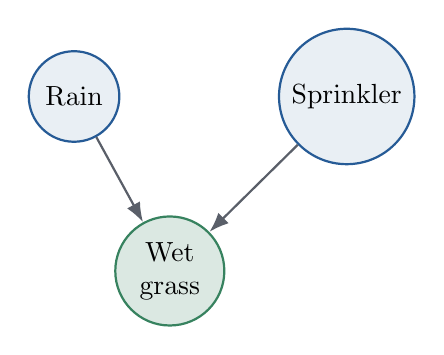
\begin{tikzpicture}[node distance=2cm]
  \node[dagNode] (rain3) {Rain};

  \node[dagNode, right=of rain3]
    (sprinkler3) {Sprinkler};

  \node[dagObserved, below right=1.3cm and 0.3cm of rain3]
    (grass3) {Wet\\grass};

  \draw[dagArrow] (rain3) -- (grass3);
  \draw[dagArrow] (sprinkler3) -- (grass3);
\end{tikzpicture}
\end{center}

Bayes' rule updates our beliefs:

\[
P(R,S\mid W)
\propto
P(W\mid R,S)P(R)P(S).
\]

\begin{itemize}
  \item Wet grass raises the probability of rain.
  \item It also raises the probability that the sprinkler ran.
  \item Learning that it rained may reduce the need to explain the wet
        grass using the sprinkler.
\end{itemize}

The last effect is called \textbf{explaining away}.

\end{frame}

% ------------------------------------------------------------
\begin{frame}{Prediction, diagnosis, and intervention}

The same graph can support different kinds of questions.

\begin{description}

  \item[Prediction:]
  If it rains, how likely is wet grass?
  \[
  P(W\mid R)
  \]

  \item[Diagnosis:]
  If the grass is wet, how likely was rain?
  \[
  P(R\mid W)
  \]

  \item[Intervention:]
  What happens if we deliberately turn on the sprinkler?
  \[
  P\bigl(W\mid \operatorname{do}(S=1)\bigr)
  \]

\end{description}

The first two are probabilistic queries.

The third is causal: it changes the data-generating process instead of
merely observing it.

\end{frame}

% ------------------------------------------------------------
\begin{frame}{A decision needs more than probabilities}

A Bayesian network tells us what is uncertain and how beliefs change.

A decision problem also requires:

\begin{itemize}
  \item the available \textbf{actions};
  \item the \textbf{information} available when choosing;
  \item and a definition of what outcomes are \textbf{valuable}.
\end{itemize}

\medskip

An \textbf{influence diagram} extends a Bayesian network.

\begin{center}
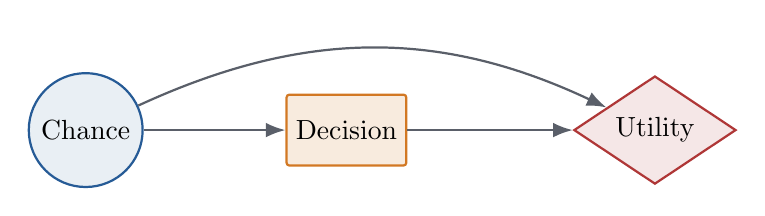
\begin{tikzpicture}[node distance=1.8cm]
  \node[dagNode] (chance) {Chance};

  \node[dagDecision, right=of chance]
    (choose) {Decision};

  \node[dagUtility, right=2.1cm of choose]
    (util) {Utility};

  \draw[dagArrow] (chance) -- (choose);
  \draw[dagArrow, bend left=25] (chance) to (util);
  \draw[dagArrow] (choose) -- (util);
\end{tikzpicture}
\end{center}

\[
\text{circles = uncertainty},\quad
\text{rectangles = choices},\quad
\text{diamonds = value}.
\]

\end{frame}

% ------------------------------------------------------------
\begin{frame}{Example: should we perform maintenance?}

\begin{center}
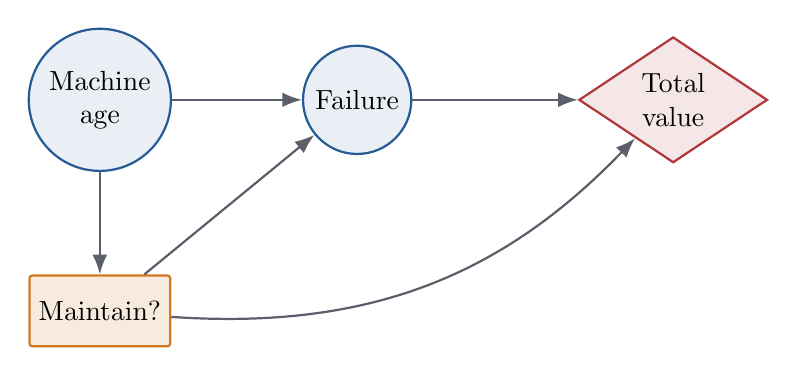
\begin{tikzpicture}[node distance=1.65cm]
  \node[dagNode] (age) {Machine\\age};

  \node[dagNode, right=of age]
    (failure) {Failure};

  \node[dagDecision, below=1.3cm of age]
    (maintain) {Maintain?};

  \node[dagUtility, right=2.1cm of failure]
    (cost) {Total\\value};

  \draw[dagArrow] (age) -- (failure);
  \draw[dagArrow] (age) -- (maintain);
  \draw[dagArrow] (maintain) -- (failure);
  \draw[dagArrow] (failure) -- (cost);
  \draw[dagArrow, bend right=25] (maintain) to (cost);
\end{tikzpicture}
\end{center}

\begin{itemize}
  \item Machine age is known before the decision.
  \item Maintenance changes the probability of failure.
  \item Maintenance costs money.
  \item Failure may cost much more.
\end{itemize}

The goal is not simply to predict failure. The goal is to choose the
action with the best expected consequences.

\end{frame}

% ------------------------------------------------------------
\begin{frame}{Expected utility: the decision rule}

Let \(d\) be a decision and let \(x\) be an uncertain outcome.

\[
EU(d)
=
\sum_x P(x\mid d,e)\,U(d,x),
\]

where \(e\) denotes the available evidence.

Choose

\[
d^*
=
\underset{d}{\operatorname{arg\,max}}\;EU(d).
\]

\begin{block}{In plain language}
For each decision:
\begin{enumerate}
  \item consider the possible outcomes;
  \item weight each outcome by its probability;
  \item attach a value to each outcome;
  \item choose the decision with the largest expected value.
\end{enumerate}
\end{block}

\end{frame}

% ------------------------------------------------------------
\begin{frame}{A small maintenance calculation}

Suppose preventive maintenance costs \$2,000.

Without maintenance:

\[
P(\text{failure})=0.20
\]

and a failure costs \$20,000.

The expected cost without maintenance is

\[
0.20(\$20{,}000)
=
\$4{,}000.
\]

If maintenance essentially prevents failure, then:

\[
\begin{aligned}
E[\text{cost}\mid\text{no maintenance}] &= \$4{,}000,\\
E[\text{cost}\mid\text{maintenance}] &= \$2{,}000.
\end{aligned}
\]

\begin{alertblock}{Decision}
On these assumptions, preventive maintenance is preferred.
\end{alertblock}

\end{frame}

% ------------------------------------------------------------
\begin{frame}{Information itself can have value}

Suppose an inspection provides information before maintenance is chosen.

\begin{center}
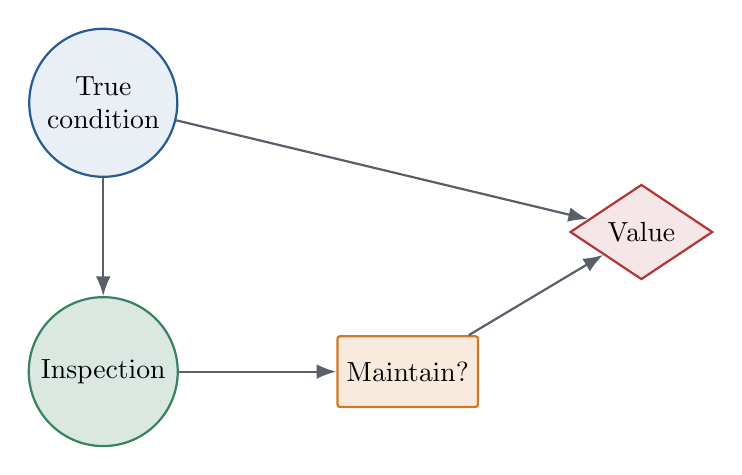
\begin{tikzpicture}[node distance=1.5cm]
  \node[dagNode] (condition) {True\\condition};

  \node[dagObserved, below=of condition]
    (inspection) {Inspection};

  \node[dagDecision, right=2cm of inspection]
    (maintenance2) {Maintain?};

  \node[dagUtility, above right=1cm and 1.6cm of maintenance2]
    (value2) {Value};

  \draw[dagArrow] (condition) -- (inspection);
  \draw[dagArrow] (condition) -- (value2);
  \draw[dagArrow] (inspection) -- (maintenance2);
  \draw[dagArrow] (maintenance2) -- (value2);
\end{tikzpicture}
\end{center}

The \textbf{value of information} is

\[
\mathrm{VOI}
=
EU(\text{best policy with information})
-
EU(\text{best policy without information}).
\]

Purchase information only when its value exceeds its cost.

\end{frame}

% ------------------------------------------------------------
\begin{frame}{A practical modeling workflow}

\begin{enumerate}
  \item Define the decision and the objective.
  \item List the relevant uncertainties and observations.
  \item Draw arrows representing direct relationships.
  \item Check that the graph is acyclic.
  \item Specify conditional probability models.
  \item Specify utilities, benefits, or costs.
  \item Enter evidence and update probabilities.
  \item Compare actions using expected utility.
  \item Test sensitivity to uncertain assumptions.
\end{enumerate}

\medskip

\begin{alertblock}{A useful modeling habit}
Start small. Add a node only when it could change beliefs, decisions,
or the interpretation of the model.
\end{alertblock}

\end{frame}

% ------------------------------------------------------------
\begin{frame}{Common pitfalls}

\begin{itemize}
  \item Treating every arrow as automatically causal
  \item Omitting an important common cause
  \item Conditioning on a collider without realizing it
  \item Adding so many variables that the model becomes unmanageable
  \item Using precise probabilities that are not well supported
  \item Optimizing predictions instead of the actual decision objective
  \item Forgetting when information becomes available
  \item Reporting one ``optimal'' answer without sensitivity analysis
\end{itemize}

\medskip

\begin{block}{A useful principle}
A good decision model should be understandable enough for its
assumptions to be questioned.
\end{block}

\end{frame}

% ------------------------------------------------------------
\begin{frame}{Takeaways}

\begin{enumerate}
  \item A DAG is a directed graph with no directed cycles.
  \item Its structure encodes relationships and possible independencies.
  \item A Bayesian network adds local probability models.
  \item Conditioning can block paths or open collider paths.
  \item An influence diagram adds decisions and utilities.
  \item Decision analysis chooses actions using expected utility, not
        probability alone.
\end{enumerate}

\bigskip

\begin{center}
\Large
DAGs turn a complicated story into a model\\
that we can inspect, calculate with, and improve.
\end{center}

\end{frame}

% ------------------------------------------------------------
%\begin{frame}{Discussion}
%
%\begin{center}
%%\Huge Questions?
%
%%\bigskip
%
%\large
%What decision problem would you represent as a DAG?
%\end{center}
%
%\end{frame}

% ============================================================
\end{document}